% Created by tikzDevice version 0.12.3.1 on 2022-07-29 15:13:42
% !TEX encoding = UTF-8 Unicode
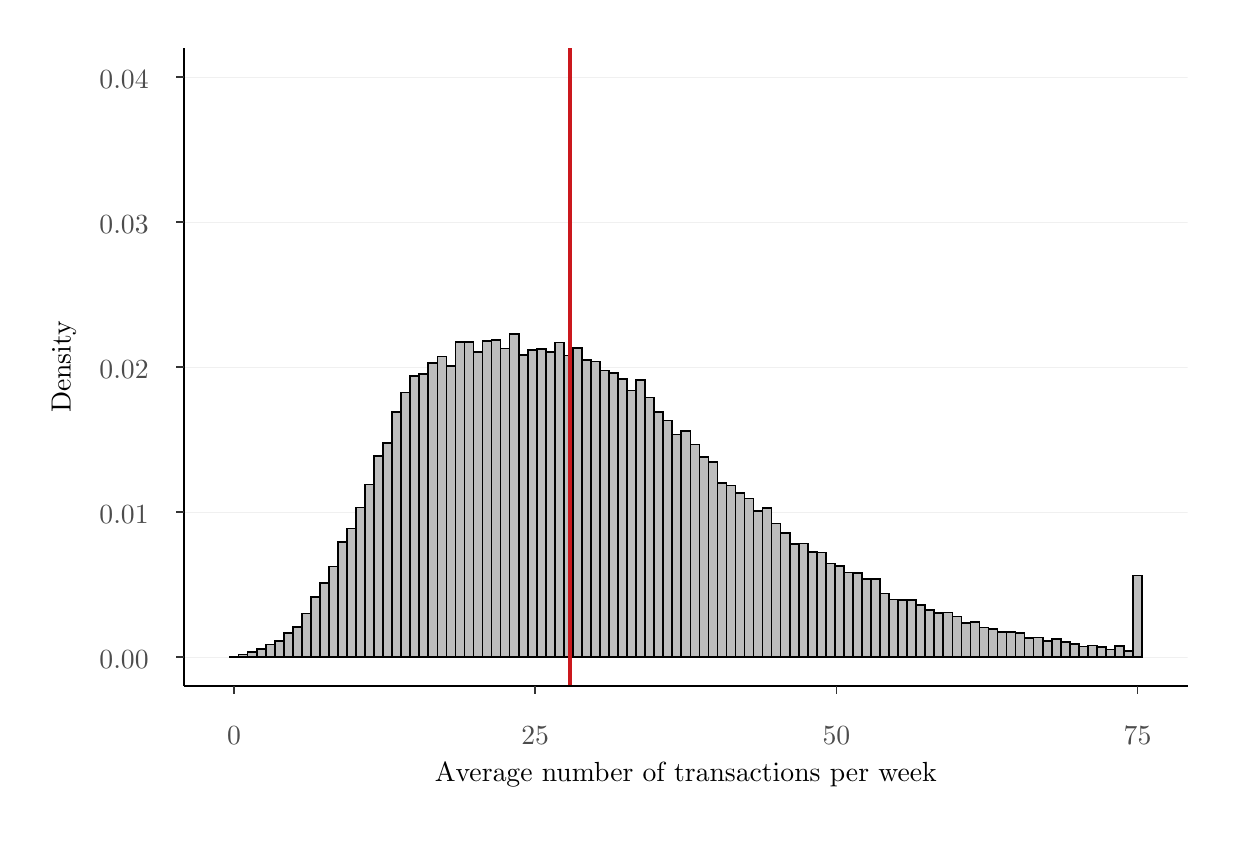
\begin{tikzpicture}[x=1pt,y=1pt]
\definecolor{fillColor}{RGB}{255,255,255}
\path[use as bounding box,fill=fillColor,fill opacity=0.00] (0,0) rectangle (433.62,289.08);
\begin{scope}
\path[clip] (  0.00,  0.00) rectangle (433.62,289.08);
\definecolor{drawColor}{RGB}{255,255,255}
\definecolor{fillColor}{RGB}{255,255,255}

\path[draw=drawColor,line width= 0.6pt,line join=round,line cap=round,fill=fillColor] ( -0.00,  0.00) rectangle (433.62,289.08);
\end{scope}
\begin{scope}
\path[clip] ( 56.47, 51.15) rectangle (419.17,281.85);
\definecolor{drawColor}{RGB}{255,255,255}

\path[draw=drawColor,line width= 0.3pt,line join=round] ( 56.47, 87.86) --
	(419.17, 87.86);

\path[draw=drawColor,line width= 0.3pt,line join=round] ( 56.47,140.29) --
	(419.17,140.29);

\path[draw=drawColor,line width= 0.3pt,line join=round] ( 56.47,192.72) --
	(419.17,192.72);

\path[draw=drawColor,line width= 0.3pt,line join=round] ( 56.47,245.15) --
	(419.17,245.15);

\path[draw=drawColor,line width= 0.3pt,line join=round] (128.99, 51.15) --
	(128.99,281.85);

\path[draw=drawColor,line width= 0.3pt,line join=round] (237.82, 51.15) --
	(237.82,281.85);

\path[draw=drawColor,line width= 0.3pt,line join=round] (346.64, 51.15) --
	(346.64,281.85);
\definecolor{drawColor}{gray}{0.94}

\path[draw=drawColor,line width= 0.1pt,line join=round] ( 56.47, 61.64) --
	(419.17, 61.64);

\path[draw=drawColor,line width= 0.1pt,line join=round] ( 56.47,114.07) --
	(419.17,114.07);

\path[draw=drawColor,line width= 0.1pt,line join=round] ( 56.47,166.50) --
	(419.17,166.50);

\path[draw=drawColor,line width= 0.1pt,line join=round] ( 56.47,218.93) --
	(419.17,218.93);

\path[draw=drawColor,line width= 0.1pt,line join=round] ( 56.47,271.37) --
	(419.17,271.37);
\definecolor{drawColor}{RGB}{0,0,0}
\definecolor{fillColor}{gray}{0.74}

\path[draw=drawColor,line width= 0.6pt,line cap=rect,fill=fillColor] ( 72.95, 61.64) rectangle ( 76.22, 61.83);

\path[draw=drawColor,line width= 0.6pt,line cap=rect,fill=fillColor] ( 76.22, 61.64) rectangle ( 79.48, 62.57);

\path[draw=drawColor,line width= 0.6pt,line cap=rect,fill=fillColor] ( 79.48, 61.64) rectangle ( 82.75, 63.50);

\path[draw=drawColor,line width= 0.6pt,line cap=rect,fill=fillColor] ( 82.75, 61.64) rectangle ( 86.01, 64.55);

\path[draw=drawColor,line width= 0.6pt,line cap=rect,fill=fillColor] ( 86.01, 61.64) rectangle ( 89.28, 66.16);

\path[draw=drawColor,line width= 0.6pt,line cap=rect,fill=fillColor] ( 89.28, 61.64) rectangle ( 92.54, 67.46);

\path[draw=drawColor,line width= 0.6pt,line cap=rect,fill=fillColor] ( 92.54, 61.64) rectangle ( 95.80, 70.31);

\path[draw=drawColor,line width= 0.6pt,line cap=rect,fill=fillColor] ( 95.80, 61.64) rectangle ( 99.07, 72.54);

\path[draw=drawColor,line width= 0.6pt,line cap=rect,fill=fillColor] ( 99.07, 61.64) rectangle (102.33, 77.43);

\path[draw=drawColor,line width= 0.6pt,line cap=rect,fill=fillColor] (102.33, 61.64) rectangle (105.60, 83.25);

\path[draw=drawColor,line width= 0.6pt,line cap=rect,fill=fillColor] (105.60, 61.64) rectangle (108.86, 88.51);

\path[draw=drawColor,line width= 0.6pt,line cap=rect,fill=fillColor] (108.86, 61.64) rectangle (112.13, 94.33);

\path[draw=drawColor,line width= 0.6pt,line cap=rect,fill=fillColor] (112.13, 61.64) rectangle (115.39,103.25);

\path[draw=drawColor,line width= 0.6pt,line cap=rect,fill=fillColor] (115.39, 61.64) rectangle (118.66,108.14);

\path[draw=drawColor,line width= 0.6pt,line cap=rect,fill=fillColor] (118.66, 61.64) rectangle (121.92,115.70);

\path[draw=drawColor,line width= 0.6pt,line cap=rect,fill=fillColor] (121.92, 61.64) rectangle (125.19,124.05);

\path[draw=drawColor,line width= 0.6pt,line cap=rect,fill=fillColor] (125.19, 61.64) rectangle (128.45,134.21);

\path[draw=drawColor,line width= 0.6pt,line cap=rect,fill=fillColor] (128.45, 61.64) rectangle (131.72,138.98);

\path[draw=drawColor,line width= 0.6pt,line cap=rect,fill=fillColor] (131.72, 61.64) rectangle (134.98,150.12);

\path[draw=drawColor,line width= 0.6pt,line cap=rect,fill=fillColor] (134.98, 61.64) rectangle (138.24,157.24);

\path[draw=drawColor,line width= 0.6pt,line cap=rect,fill=fillColor] (138.24, 61.64) rectangle (141.51,163.25);

\path[draw=drawColor,line width= 0.6pt,line cap=rect,fill=fillColor] (141.51, 61.64) rectangle (144.77,163.93);

\path[draw=drawColor,line width= 0.6pt,line cap=rect,fill=fillColor] (144.77, 61.64) rectangle (148.04,167.89);

\path[draw=drawColor,line width= 0.6pt,line cap=rect,fill=fillColor] (148.04, 61.64) rectangle (151.30,170.31);

\path[draw=drawColor,line width= 0.6pt,line cap=rect,fill=fillColor] (151.30, 61.64) rectangle (154.57,166.78);

\path[draw=drawColor,line width= 0.6pt,line cap=rect,fill=fillColor] (154.57, 61.64) rectangle (157.83,175.45);

\path[draw=drawColor,line width= 0.6pt,line cap=rect,fill=fillColor] (157.83, 61.64) rectangle (161.10,175.38);

\path[draw=drawColor,line width= 0.6pt,line cap=rect,fill=fillColor] (161.10, 61.64) rectangle (164.36,171.98);

\path[draw=drawColor,line width= 0.6pt,line cap=rect,fill=fillColor] (164.36, 61.64) rectangle (167.63,175.88);

\path[draw=drawColor,line width= 0.6pt,line cap=rect,fill=fillColor] (167.63, 61.64) rectangle (170.89,176.25);

\path[draw=drawColor,line width= 0.6pt,line cap=rect,fill=fillColor] (170.89, 61.64) rectangle (174.16,173.09);

\path[draw=drawColor,line width= 0.6pt,line cap=rect,fill=fillColor] (174.16, 61.64) rectangle (177.42,178.42);

\path[draw=drawColor,line width= 0.6pt,line cap=rect,fill=fillColor] (177.42, 61.64) rectangle (180.68,170.86);

\path[draw=drawColor,line width= 0.6pt,line cap=rect,fill=fillColor] (180.68, 61.64) rectangle (183.95,172.66);

\path[draw=drawColor,line width= 0.6pt,line cap=rect,fill=fillColor] (183.95, 61.64) rectangle (187.21,172.97);

\path[draw=drawColor,line width= 0.6pt,line cap=rect,fill=fillColor] (187.21, 61.64) rectangle (190.48,171.92);

\path[draw=drawColor,line width= 0.6pt,line cap=rect,fill=fillColor] (190.48, 61.64) rectangle (193.74,175.26);

\path[draw=drawColor,line width= 0.6pt,line cap=rect,fill=fillColor] (193.74, 61.64) rectangle (197.01,170.62);

\path[draw=drawColor,line width= 0.6pt,line cap=rect,fill=fillColor] (197.01, 61.64) rectangle (200.27,173.40);

\path[draw=drawColor,line width= 0.6pt,line cap=rect,fill=fillColor] (200.27, 61.64) rectangle (203.54,168.88);

\path[draw=drawColor,line width= 0.6pt,line cap=rect,fill=fillColor] (203.54, 61.64) rectangle (206.80,168.45);

\path[draw=drawColor,line width= 0.6pt,line cap=rect,fill=fillColor] (206.80, 61.64) rectangle (210.07,165.17);

\path[draw=drawColor,line width= 0.6pt,line cap=rect,fill=fillColor] (210.07, 61.64) rectangle (213.33,164.36);

\path[draw=drawColor,line width= 0.6pt,line cap=rect,fill=fillColor] (213.33, 61.64) rectangle (216.60,162.07);

\path[draw=drawColor,line width= 0.6pt,line cap=rect,fill=fillColor] (216.60, 61.64) rectangle (219.86,157.92);

\path[draw=drawColor,line width= 0.6pt,line cap=rect,fill=fillColor] (219.86, 61.64) rectangle (223.13,161.76);

\path[draw=drawColor,line width= 0.6pt,line cap=rect,fill=fillColor] (223.13, 61.64) rectangle (226.39,155.39);

\path[draw=drawColor,line width= 0.6pt,line cap=rect,fill=fillColor] (226.39, 61.64) rectangle (229.65,150.31);

\path[draw=drawColor,line width= 0.6pt,line cap=rect,fill=fillColor] (229.65, 61.64) rectangle (232.92,147.09);

\path[draw=drawColor,line width= 0.6pt,line cap=rect,fill=fillColor] (232.92, 61.64) rectangle (236.18,142.13);

\path[draw=drawColor,line width= 0.6pt,line cap=rect,fill=fillColor] (236.18, 61.64) rectangle (239.45,143.43);

\path[draw=drawColor,line width= 0.6pt,line cap=rect,fill=fillColor] (239.45, 61.64) rectangle (242.71,138.48);

\path[draw=drawColor,line width= 0.6pt,line cap=rect,fill=fillColor] (242.71, 61.64) rectangle (245.98,133.84);

\path[draw=drawColor,line width= 0.6pt,line cap=rect,fill=fillColor] (245.98, 61.64) rectangle (249.24,132.23);

\path[draw=drawColor,line width= 0.6pt,line cap=rect,fill=fillColor] (249.24, 61.64) rectangle (252.51,124.55);

\path[draw=drawColor,line width= 0.6pt,line cap=rect,fill=fillColor] (252.51, 61.64) rectangle (255.77,123.62);

\path[draw=drawColor,line width= 0.6pt,line cap=rect,fill=fillColor] (255.77, 61.64) rectangle (259.04,121.02);

\path[draw=drawColor,line width= 0.6pt,line cap=rect,fill=fillColor] (259.04, 61.64) rectangle (262.30,118.91);

\path[draw=drawColor,line width= 0.6pt,line cap=rect,fill=fillColor] (262.30, 61.64) rectangle (265.57,114.39);

\path[draw=drawColor,line width= 0.6pt,line cap=rect,fill=fillColor] (265.57, 61.64) rectangle (268.83,115.45);

\path[draw=drawColor,line width= 0.6pt,line cap=rect,fill=fillColor] (268.83, 61.64) rectangle (272.09,109.94);

\path[draw=drawColor,line width= 0.6pt,line cap=rect,fill=fillColor] (272.09, 61.64) rectangle (275.36,106.53);

\path[draw=drawColor,line width= 0.6pt,line cap=rect,fill=fillColor] (275.36, 61.64) rectangle (278.62,102.51);

\path[draw=drawColor,line width= 0.6pt,line cap=rect,fill=fillColor] (278.62, 61.64) rectangle (281.89,102.69);

\path[draw=drawColor,line width= 0.6pt,line cap=rect,fill=fillColor] (281.89, 61.64) rectangle (285.15, 99.60);

\path[draw=drawColor,line width= 0.6pt,line cap=rect,fill=fillColor] (285.15, 61.64) rectangle (288.42, 99.47);

\path[draw=drawColor,line width= 0.6pt,line cap=rect,fill=fillColor] (288.42, 61.64) rectangle (291.68, 95.51);

\path[draw=drawColor,line width= 0.6pt,line cap=rect,fill=fillColor] (291.68, 61.64) rectangle (294.95, 94.52);

\path[draw=drawColor,line width= 0.6pt,line cap=rect,fill=fillColor] (294.95, 61.64) rectangle (298.21, 92.23);

\path[draw=drawColor,line width= 0.6pt,line cap=rect,fill=fillColor] (298.21, 61.64) rectangle (301.48, 92.10);

\path[draw=drawColor,line width= 0.6pt,line cap=rect,fill=fillColor] (301.48, 61.64) rectangle (304.74, 89.81);

\path[draw=drawColor,line width= 0.6pt,line cap=rect,fill=fillColor] (304.74, 61.64) rectangle (308.01, 89.75);

\path[draw=drawColor,line width= 0.6pt,line cap=rect,fill=fillColor] (308.01, 61.64) rectangle (311.27, 84.61);

\path[draw=drawColor,line width= 0.6pt,line cap=rect,fill=fillColor] (311.27, 61.64) rectangle (314.53, 82.51);

\path[draw=drawColor,line width= 0.6pt,line cap=rect,fill=fillColor] (314.53, 61.64) rectangle (317.80, 82.26);

\path[draw=drawColor,line width= 0.6pt,line cap=rect,fill=fillColor] (317.80, 61.64) rectangle (321.06, 82.32);

\path[draw=drawColor,line width= 0.6pt,line cap=rect,fill=fillColor] (321.06, 61.64) rectangle (324.33, 80.46);

\path[draw=drawColor,line width= 0.6pt,line cap=rect,fill=fillColor] (324.33, 61.64) rectangle (327.59, 78.54);

\path[draw=drawColor,line width= 0.6pt,line cap=rect,fill=fillColor] (327.59, 61.64) rectangle (330.86, 77.55);

\path[draw=drawColor,line width= 0.6pt,line cap=rect,fill=fillColor] (330.86, 61.64) rectangle (334.12, 77.74);

\path[draw=drawColor,line width= 0.6pt,line cap=rect,fill=fillColor] (334.12, 61.64) rectangle (337.39, 76.25);

\path[draw=drawColor,line width= 0.6pt,line cap=rect,fill=fillColor] (337.39, 61.64) rectangle (340.65, 73.96);

\path[draw=drawColor,line width= 0.6pt,line cap=rect,fill=fillColor] (340.65, 61.64) rectangle (343.92, 74.33);

\path[draw=drawColor,line width= 0.6pt,line cap=rect,fill=fillColor] (343.92, 61.64) rectangle (347.18, 72.29);

\path[draw=drawColor,line width= 0.6pt,line cap=rect,fill=fillColor] (347.18, 61.64) rectangle (350.45, 71.73);

\path[draw=drawColor,line width= 0.6pt,line cap=rect,fill=fillColor] (350.45, 61.64) rectangle (353.71, 70.80);

\path[draw=drawColor,line width= 0.6pt,line cap=rect,fill=fillColor] (353.71, 61.64) rectangle (356.97, 70.62);

\path[draw=drawColor,line width= 0.6pt,line cap=rect,fill=fillColor] (356.97, 61.64) rectangle (360.24, 70.31);

\path[draw=drawColor,line width= 0.6pt,line cap=rect,fill=fillColor] (360.24, 61.64) rectangle (363.50, 68.45);

\path[draw=drawColor,line width= 0.6pt,line cap=rect,fill=fillColor] (363.50, 61.64) rectangle (366.77, 68.70);

\path[draw=drawColor,line width= 0.6pt,line cap=rect,fill=fillColor] (366.77, 61.64) rectangle (370.03, 67.52);

\path[draw=drawColor,line width= 0.6pt,line cap=rect,fill=fillColor] (370.03, 61.64) rectangle (373.30, 68.20);

\path[draw=drawColor,line width= 0.6pt,line cap=rect,fill=fillColor] (373.30, 61.64) rectangle (376.56, 67.09);

\path[draw=drawColor,line width= 0.6pt,line cap=rect,fill=fillColor] (376.56, 61.64) rectangle (379.83, 66.47);

\path[draw=drawColor,line width= 0.6pt,line cap=rect,fill=fillColor] (379.83, 61.64) rectangle (383.09, 65.48);

\path[draw=drawColor,line width= 0.6pt,line cap=rect,fill=fillColor] (383.09, 61.64) rectangle (386.36, 65.85);

\path[draw=drawColor,line width= 0.6pt,line cap=rect,fill=fillColor] (386.36, 61.64) rectangle (389.62, 65.17);

\path[draw=drawColor,line width= 0.6pt,line cap=rect,fill=fillColor] (389.62, 61.64) rectangle (392.89, 64.43);

\path[draw=drawColor,line width= 0.6pt,line cap=rect,fill=fillColor] (392.89, 61.64) rectangle (396.15, 65.60);

\path[draw=drawColor,line width= 0.6pt,line cap=rect,fill=fillColor] (396.15, 61.64) rectangle (399.41, 63.87);

\path[draw=drawColor,line width= 0.6pt,line cap=rect,fill=fillColor] (399.41, 61.64) rectangle (402.68, 91.11);
\definecolor{drawColor}{RGB}{203,24,29}

\path[draw=drawColor,line width= 1.7pt,line join=round] (195.96, 51.15) -- (195.96,281.85);
\end{scope}
\begin{scope}
\path[clip] (  0.00,  0.00) rectangle (433.62,289.08);
\definecolor{drawColor}{RGB}{0,0,0}

\path[draw=drawColor,line width= 0.6pt,line join=round] ( 56.47, 51.15) --
	( 56.47,281.85);
\end{scope}
\begin{scope}
\path[clip] (  0.00,  0.00) rectangle (433.62,289.08);
\definecolor{drawColor}{gray}{0.30}

\node[text=drawColor,anchor=base east,inner sep=0pt, outer sep=0pt, scale=  1.00] at ( 43.72, 57.51) {0.00};

\node[text=drawColor,anchor=base east,inner sep=0pt, outer sep=0pt, scale=  1.00] at ( 43.72,109.94) {0.01};

\node[text=drawColor,anchor=base east,inner sep=0pt, outer sep=0pt, scale=  1.00] at ( 43.72,162.37) {0.02};

\node[text=drawColor,anchor=base east,inner sep=0pt, outer sep=0pt, scale=  1.00] at ( 43.72,214.80) {0.03};

\node[text=drawColor,anchor=base east,inner sep=0pt, outer sep=0pt, scale=  1.00] at ( 43.72,267.23) {0.04};
\end{scope}
\begin{scope}
\path[clip] (  0.00,  0.00) rectangle (433.62,289.08);
\definecolor{drawColor}{gray}{0.20}

\path[draw=drawColor,line width= 0.6pt,line join=round] ( 53.72, 61.64) --
	( 56.47, 61.64);

\path[draw=drawColor,line width= 0.6pt,line join=round] ( 53.72,114.07) --
	( 56.47,114.07);

\path[draw=drawColor,line width= 0.6pt,line join=round] ( 53.72,166.50) --
	( 56.47,166.50);

\path[draw=drawColor,line width= 0.6pt,line join=round] ( 53.72,218.93) --
	( 56.47,218.93);

\path[draw=drawColor,line width= 0.6pt,line join=round] ( 53.72,271.37) --
	( 56.47,271.37);
\end{scope}
\begin{scope}
\path[clip] (  0.00,  0.00) rectangle (433.62,289.08);
\definecolor{drawColor}{RGB}{0,0,0}

\path[draw=drawColor,line width= 0.6pt,line join=round] ( 56.47, 51.15) --
	(419.17, 51.15);
\end{scope}
\begin{scope}
\path[clip] (  0.00,  0.00) rectangle (433.62,289.08);
\definecolor{drawColor}{gray}{0.20}

\path[draw=drawColor,line width= 0.6pt,line join=round] ( 74.58, 48.40) --
	( 74.58, 51.15);

\path[draw=drawColor,line width= 0.6pt,line join=round] (183.41, 48.40) --
	(183.41, 51.15);

\path[draw=drawColor,line width= 0.6pt,line join=round] (292.23, 48.40) --
	(292.23, 51.15);

\path[draw=drawColor,line width= 0.6pt,line join=round] (401.05, 48.40) --
	(401.05, 51.15);
\end{scope}
\begin{scope}
\path[clip] (  0.00,  0.00) rectangle (433.62,289.08);
\definecolor{drawColor}{gray}{0.30}

\node[text=drawColor,anchor=base,inner sep=0pt, outer sep=0pt, scale=  1.00] at ( 74.58, 30.14) {0};

\node[text=drawColor,anchor=base,inner sep=0pt, outer sep=0pt, scale=  1.00] at (183.41, 30.14) {25};

\node[text=drawColor,anchor=base,inner sep=0pt, outer sep=0pt, scale=  1.00] at (292.23, 30.14) {50};

\node[text=drawColor,anchor=base,inner sep=0pt, outer sep=0pt, scale=  1.00] at (401.05, 30.14) {75};
\end{scope}
\begin{scope}
\path[clip] (  0.00,  0.00) rectangle (433.62,289.08);
\definecolor{drawColor}{RGB}{0,0,0}

\node[text=drawColor,anchor=base,inner sep=0pt, outer sep=0pt, scale=  1.00] at (237.82, 16.79) {Average number of transactions per week};
\end{scope}
\begin{scope}
\path[clip] (  0.00,  0.00) rectangle (433.62,289.08);
\definecolor{drawColor}{RGB}{0,0,0}

\node[text=drawColor,rotate= 90.00,anchor=base,inner sep=0pt, outer sep=0pt, scale=  1.00] at ( 15.49,166.50) {Density};
\end{scope}
\end{tikzpicture}
